%***************************************PREAMBLE***************************************
\documentclass[a4paper,12pt]{article}

\usepackage[utf8]{inputenc}
\usepackage[margin=0.7in]{geometry}
\usepackage[T1]{fontenc}
\usepackage{graphicx}
\usepackage{float}
\usepackage{setspace}
\usepackage{appendix}
\usepackage{amsmath}
\usepackage{amssymb}
\usepackage{cite}
\usepackage{caption}
\usepackage{subcaption}


%***************************************DOCUMENT***************************************

\DeclareMathOperator*{\argmin}{\arg\!\min}
\DeclareMathOperator*{\argmax}{\arg\!\max}

\graphicspath{ {./images/} }
\setlength{\parindent}{0pt}

\begin{document}
	\fontfamily{ptm}\selectfont
	%%%%%%%%%%%%%%%%%%%%%%%%%%%%%%%%%%%%%%%COVERSHEET%%%%%%%%%%%%%%%%%%%%%%%%%%%%%%%%%%%%%%%
	\begin{titlepage}
		\setlength{\voffset}{-0.8in}
		\noindent \makebox[\textwidth]{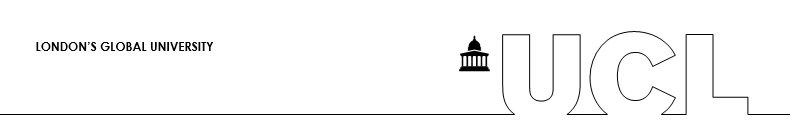
\includegraphics[width=1.2\textwidth]{Coversheet_Header.png}}
	
			\vspace{15mm}
			
			\begin{center}
				{\Huge \textbf{COMP0037 \\ \vspace{10mm} Report}}
			
				\vspace{8mm}
			
				\begin{spacing}{1.8}
					{\huge Planning in Uncertain Worlds}
				\end{spacing}
		
			
				\vspace{12mm}
			
				{\LARGE \textbf{Group AS}}
				
				\vspace{10mm}
				
				\begin{tabular}{ll}
					\underline{\textbf{Student Name}}  & \hspace{4mm} \underline{\textbf{Student number}} \vspace{2mm} \\
					Arundathi Shaji Shanthini & \hspace{4mm} 16018351 \\ 
					Dmitry Leyko & \hspace{4mm}  16021440\\ 
					Tharmetharan Balendran & \hspace{4mm} 17011729\\ 
				\end{tabular}
				
				\vspace{13mm}
				
				\begin{tabular}{ll}
					\textbf{Department:} &  Department of Electronic and Electrical Engineering\\ \vspace{3mm}
					\textbf{Submission Date:} &  28\textsuperscript{th} of April 2020
				\end{tabular}
			\end{center}
	\end{titlepage}
	%%%%%%%%%%%%%%%%%%%%%%%%%%%%%%%%%%%%%%
	
	\pagebreak
	
	\tableofcontents
	
	\pagebreak
	
	%%%%%%%%%%% PART 1 %%%%%%%%%%%%%%%%%
	\section{Decision Re-Plan Policy}

		\subsection{Policy Selection when Obstacle is Observed}
			
			\begin{figure}[H]
				\centering
				\begin{subfigure}{.4\textwidth}
					\centering
					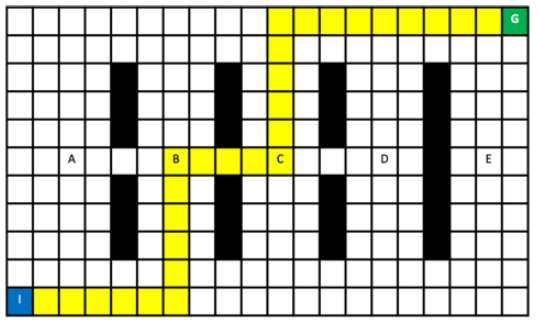
\includegraphics[width=\linewidth]{originalPlannedPath.png}
					\caption{The original planned path form I to G going through Aisle B and C.}
					\label{fig:originalPlannedPath}
				\end{subfigure}
				\begin{subfigure}{.4\textwidth}
					\centering
					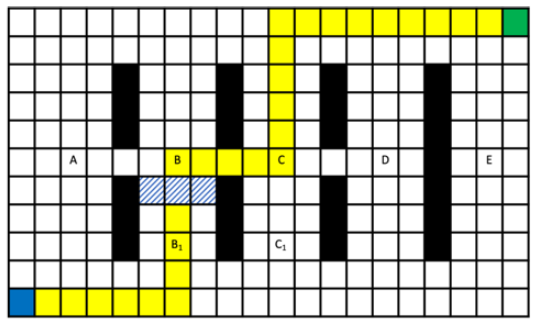
\includegraphics[width=\linewidth]{blockedAisleB.png}
					\caption{An obstacle in aisle B obstructs the planned path of the robot.}
					\label{fig:blockedAisleB}
				\end{subfigure}
				\caption{Illustration of case where robot observes an obstruction to it's planned path.}
				\label{fig:task1_1Figures}
			\end{figure}

			The scenario that we will be analysing is the case shown in Fig. \ref{fig:originalPlannedPath}. The robot is required to go from a cell $I$ to a cell $G$. These cells are marked blue and green in Fig. \ref{fig:originalPlannedPath} respectively. The figure also shows the original planned path that the robot computed going down aisle B. However, once the robot turns into aisle B it observes that the aisle is blocked. This observation is done at the point when the robot reaches the cell labelled $B_{1}$. At this point the robot can either decide to wait until the obstruction clears or it can re-plan a path. Once the robot observes the obstacle, the time the robot must wait for the obstacle to clear may be represented by the expression in Eq. \ref{eq:waitTime}. 

			\begin{equation}
				T=\frac{0.5}{\lambda_{B}}+\widetilde{T}
				\label{eq:waitTime}
			\end{equation}

			The wait time is dependent on $\lambda_{B}$ and a random variable $\widetilde{T}$. The random variable $\widetilde{T}$ is sampled from a exponential distribution with a rate parameter of $0.5\lambda_{B}$. The probability density function (PDF) for $\widetilde{T}$ is shown in Eq. \ref{eq:waitTimePDF}. 

			\begin{equation}
				f(t) = \left\{
				\begin{array}{ll}
					0.5\lambda_{B} e^{-0.5\lambda_{B} t} & \quad t \geq 0 \\
					0 & \quad t < 0
				\end{array}
				\right.
				\label{eq:waitTimePDF}
			\end{equation}

			As previously mentioned, the robot has two options to choose from: to wait for the obstacle to clear, or to re-plan and execute the new path. The two are different policies the robot must choose from. We use the symbol $\pi$ to denote a policy. A policy is a mapping from the world state to an action the robot can execute.
			\\
			\\
			Let us assume that if the robot decides to wait the total path length (number of cells) will be $K_1$ while if the robot decides to re-plan and execute the total path length will be $K_2$. We let the quantity $K$ equal to the larger value between $K_1$ and $K_2$. Now we may write the policy for the robot to wait as $\pi_{K}^{1}$ and the policy for re-planning as $\pi_{K}^{2}$. These policies are padded correspondingly to produce actions $\textbf{u}_{K}^{1}$ and $\textbf{u}_{K}^{1}$ that are padded with zero-cost state preserving actions.
			\\
			\\
			To see which policy is better on average, we consider the expected value of the cost function for both cases. The case when policy $\pi_{K}^{1}$ is chosen is characterized by the inequality shown in Eq. \ref{eq:costExpectation}.

			\begin{equation}
				\mathbb{E}\left[L\left(\pi_{K}^{1}\right)\right] \leq \mathbb{E}\left[L\left(\pi_{K}^{2}\right)\right]
				\label{eq:costExpectation}
			\end{equation}

			\begin{figure}[H]
				\centering
				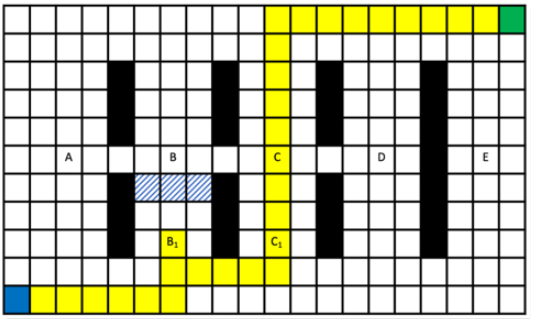
\includegraphics[scale=0.6]{images/replannedPathAisleB.png}
				\caption{The path for the re-plan policy $\pi_{K}^{2}$ which bypasses aisle B and goes down aisle C.}
				\label{fig:replannedPathAisleB}
			\end{figure}

			We can see from Fig. \ref{fig:originalPlannedPath} that the cost of the original planned path is given by the expression in Eq. \ref{eq:waitingPolicyCost}. In this equation, the terms $L_{XY}$ denote the cost of the shortest path between cell $X$ and cell $Y$. Additionally, the term $L_{W}$ represents the cost of waiting 1 unit of time.
			
			\begin{equation}
				L\left(\pi_{K}^{1}\right) = L_{IB_{1}} + TL_W + L_{B_{1}B} + L_{BC} + L_{CG}
				\label{eq:waitingPolicyCost}
			\end{equation}

			From Fig. \ref{fig:replannedPathAisleB} which shows the re-planned path, we can also see that the cost of this path is equal to the expression in Eq. \ref{eq:replanPolicyCost}

			\begin{equation}
				L\left(\pi_{K}^{2}\right) = L_{IB_{1}} + L_{B_{1}C_{1}} + L_{C_{1}C} + L_{CG}
				\label{eq:replanPolicyCost}
			\end{equation}

			Substituting the expressions in Eq. \ref{eq:waitingPolicyCost} and Eq. \ref{eq:replanPolicyCost} into Eq. \ref{eq:costExpectation}. We obtain the inequality shown in Eq. \ref{eq:costExpectation1}

			\begin{equation}
				\begin{split}
					\mathbb{E}\left[L_{IB_{1}} + TL_W + L_{B_{1}B} + L_{BC} + L_{CG}\right] & \leq \mathbb{E}\left[L_{IB_{1}} + L_{B_{1}C_{1}} + L_{C_{1}C} + L_{CG}\right] \\
					L_{IB_{1}} + \mathbb{E}\left[T\right] L_W + L_{B_{1}B} + L_{BC} + L_{CG} & \leq L_{IB_{1}} + L_{B_{1}C_{1}} + L_{C_{1}C} + L_{CG} \\
					\mathbb{E}\left[T\right] & \leq \frac{L_{B_{1}C_{1}} + L_{C_{1}C} - L_{B_{1}B} - L_{BC}}{L_W}
				\end{split}
				\label{eq:costExpectation1}
			\end{equation}

			The quantity $\mathbb{E}\left[T\right]$ is the expected value for the time the robot has to wait for the obstacle to clear. As we know the distribution that the variable is sampled from we can compute the expected value. The expected value for the time taken is given by the expression found in Eq. \ref{eq:waitTimeExpectation}

			\begin{equation}
				\begin{split}
					\mathbb{E}\left[T\right] & = \mathbb{E}\left[\frac{0.5}{\lambda_{B}}+\widetilde{T}\right] \\
					& = \frac{0.5}{\lambda_{B}} + \mathbb{E}\left[\widetilde{T}\right] \\
					& = \frac{0.5}{\lambda_{B}} + \int_{0}^{\infty}t0.5\lambda_{B}e^{0.5\lambda_{B}t} dt \\
					& = \frac{0.5}{\lambda_{B}} + \left[\left(t\right) \left(-e^{0.5\lambda_{B}t}\right)\right]_{0}^{\infty} - \int_{0}^{\infty}e^{0.5\lambda_{B}t} dt \\
					& = \frac{0.5}{\lambda_{B}} + \left[-te^{0.5\lambda_{B}t}\right]_{0}^{\infty} - \left[-\frac{1}{0.5\lambda_{B}}e^{0.5\lambda_{B}t}\right]_{0}^{\infty} \\
					& = \frac{0.5}{\lambda_{B}} + \left[-te^{0.5\lambda_{B}t} + \frac{1}{0.5\lambda_{B}}e^{0.5\lambda_{B}t}\right]_{0}^{\infty} \\
					& = \frac{0.5}{\lambda_{B}} + \lim_{x \to +\infty} \left[-te^{0.5\lambda_{B}t} + \frac{1}{0.5\lambda_{B}}e^{0.5\lambda_{B}t}\right] + \frac{1}{0.5\lambda_{B}} \\
					& = \frac{0.5}{\lambda_{B}} + \frac{1}{0.5\lambda_{B}} = \frac{2.5}{\lambda_{B}}
				\end{split}
				\label{eq:waitTimeExpectation}
			\end{equation}

			Substituting the expression from Eq. \ref{eq:waitTimeExpectation} into Eq. \ref{eq:costExpectation1} we obtain the expression in Eq. \ref{eq:lambdaInequality}. The right-hand side of the inequality in Eq. \ref{eq:lambdaInequality} represents the smallest possible value for $\lambda_{B}$ for which the waiting policy $\pi_K^1$ is a better option than the re-plan policy $\pi_K^2$. The inequality also takes into consideration the constraint that $\lambda_{B} > 0$ and negates the solution when $\lambda_{B} < 0$.

			\begin{equation}
				\begin{split}
					\frac{2.5}{\lambda_{B}} & \leq \frac{L_{B_{1}C_{1}} + L_{C_{1}C} - L_{B_{1}B} - L_{BC}}{L_W} \\
					\lambda_{B} & \geq \frac{2.5L_W}{L_{B_{1}C_{1}} + L_{C_{1}C} - L_{B_{1}B} - L_{BC}}
				\end{split}
				\label{eq:lambdaInequality}
			\end{equation}

		\subsection{Policy Selection at Start}

		\subsection{Considering the Probability of the Obstacle Being Present}

		\subsection{Considering Multiple Obstacles}

	%%%%%%%%%%%%%%%%%%%%%%%%%%%%%%%%%%%%%%
	
	%%%%%%%%%%% PART 2 %%%%%%%%%%%%%%%%%
	\section{Implementation of the System in ROS}
	\subsection{Planning path via an Aisle}
	In the given map of the environment (Fig. \ref{fig:originalPlannedPath}), we can see that the map has 5 labelled aisles - A, B, C, D and E. For the given system, it might be desirable to be able to control the path planning such that the planned path goes down an aisle. 
	
	To implement this system, the function \textit{planPathToGoalViaAisle()} in \textit{comp0037\textunderscore reactive\textunderscore planner\textunderscore controller\slash src\slash reactive\textunderscore planner\textunderscore controller.py} was completed. To ensure that the path planned goes down a particular aisle, a multiple destination path planning approach was adopted such that the first destination is the mid point\footnote{The walls dividing the aisles are disjoint in the middle this means that choosing the mid point would ensure this algorithm does not result in adding to a higher cost than is required to be able to plan a via an aisle. Hence, the mid point was chosen.} of the aisle the path has go down and the second and final destination is the goal.
	The function \textit{planPathToGoalViaAisle()} first checks to see if the class variable \textit{aisleToDriveDown} is None. If this is true, it assigns the value of the function parameter \textbf{aisle} to \textbf{aisleToDriveDown} and then the coordinates of the midpoint of the aisle is found. Once, the aisle cell coordinates are obtained path planning is done by calling \textbf{planner.search} twice. First the path is planned from the starting cell (\textit{startCellCoords}) to the mid point of the aisle (\textit{aisleCellCoords}). Then, a path is planned from the mid point of the aisle(\textit{aisleCellCoords}) to the goal cell (\textit{goalCellCoords}). Finally, the two individual paths are concatenated together and the concatenated path is plotted on search grid so that the resulting planned path can be observed.

	The resulting search grid to demonstrate the performance of this function can be seen in Fig. \ref{fig:result-of-plan-via-aisle} below.
	\begin{figure}[htp]
		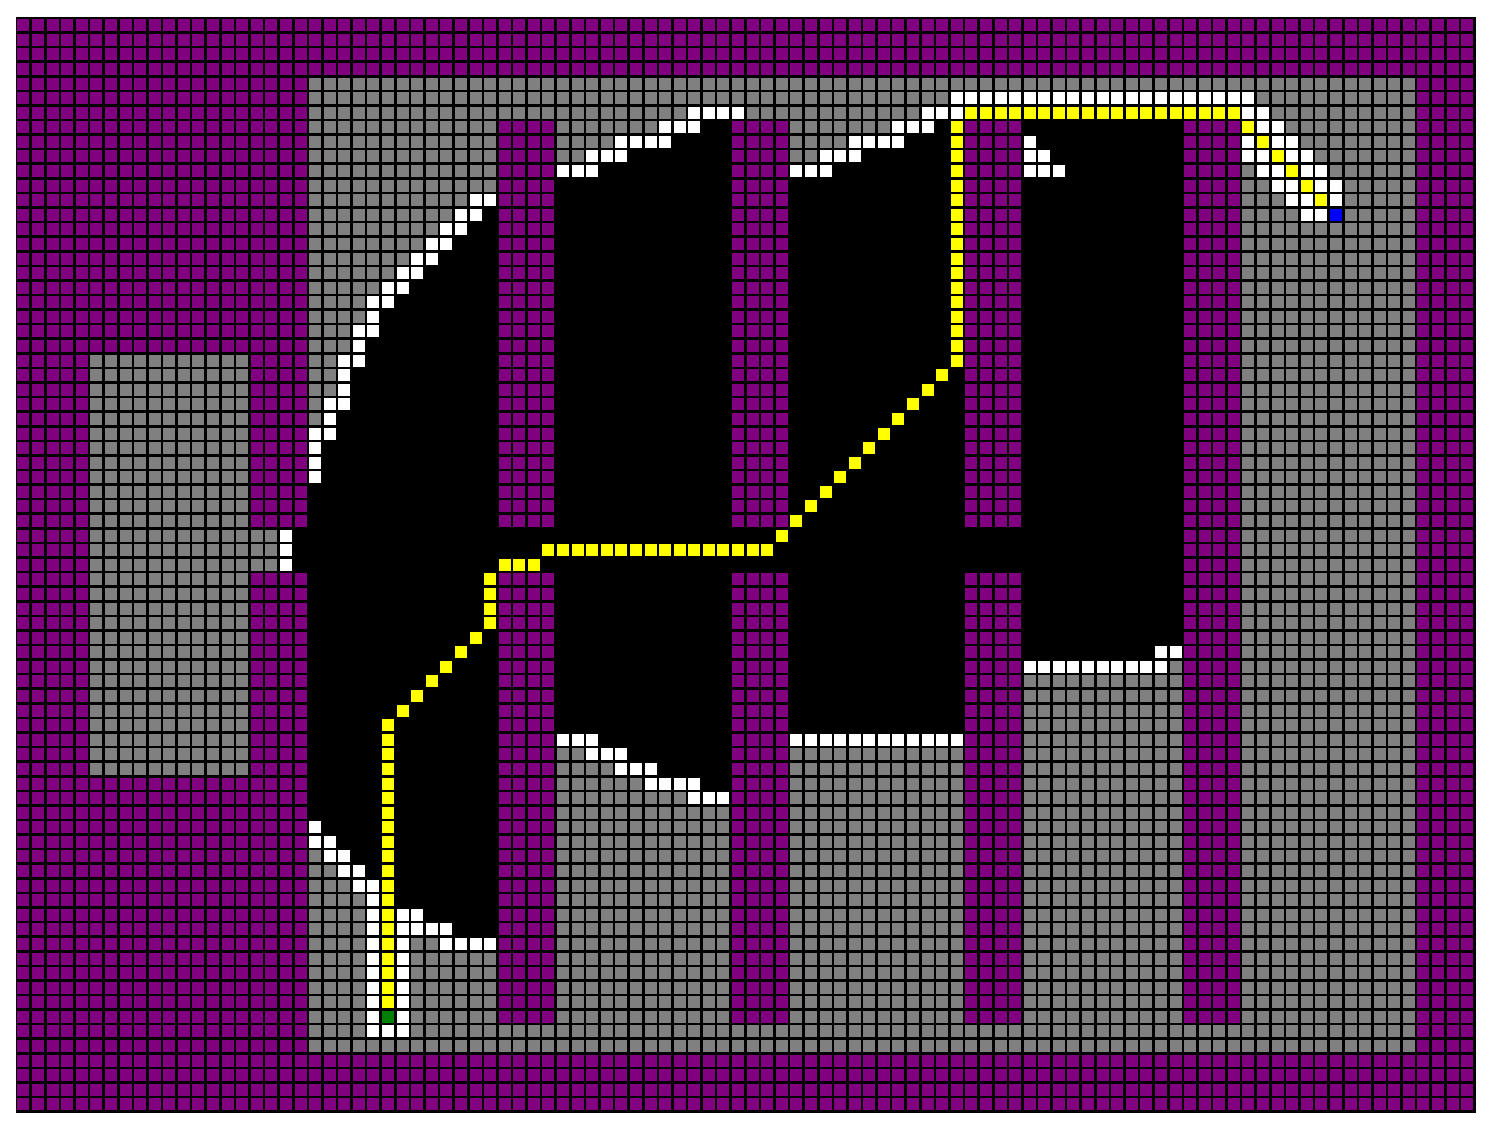
\includegraphics[width=.5\textwidth]{../exports/initial_search_grid_aisleA}
		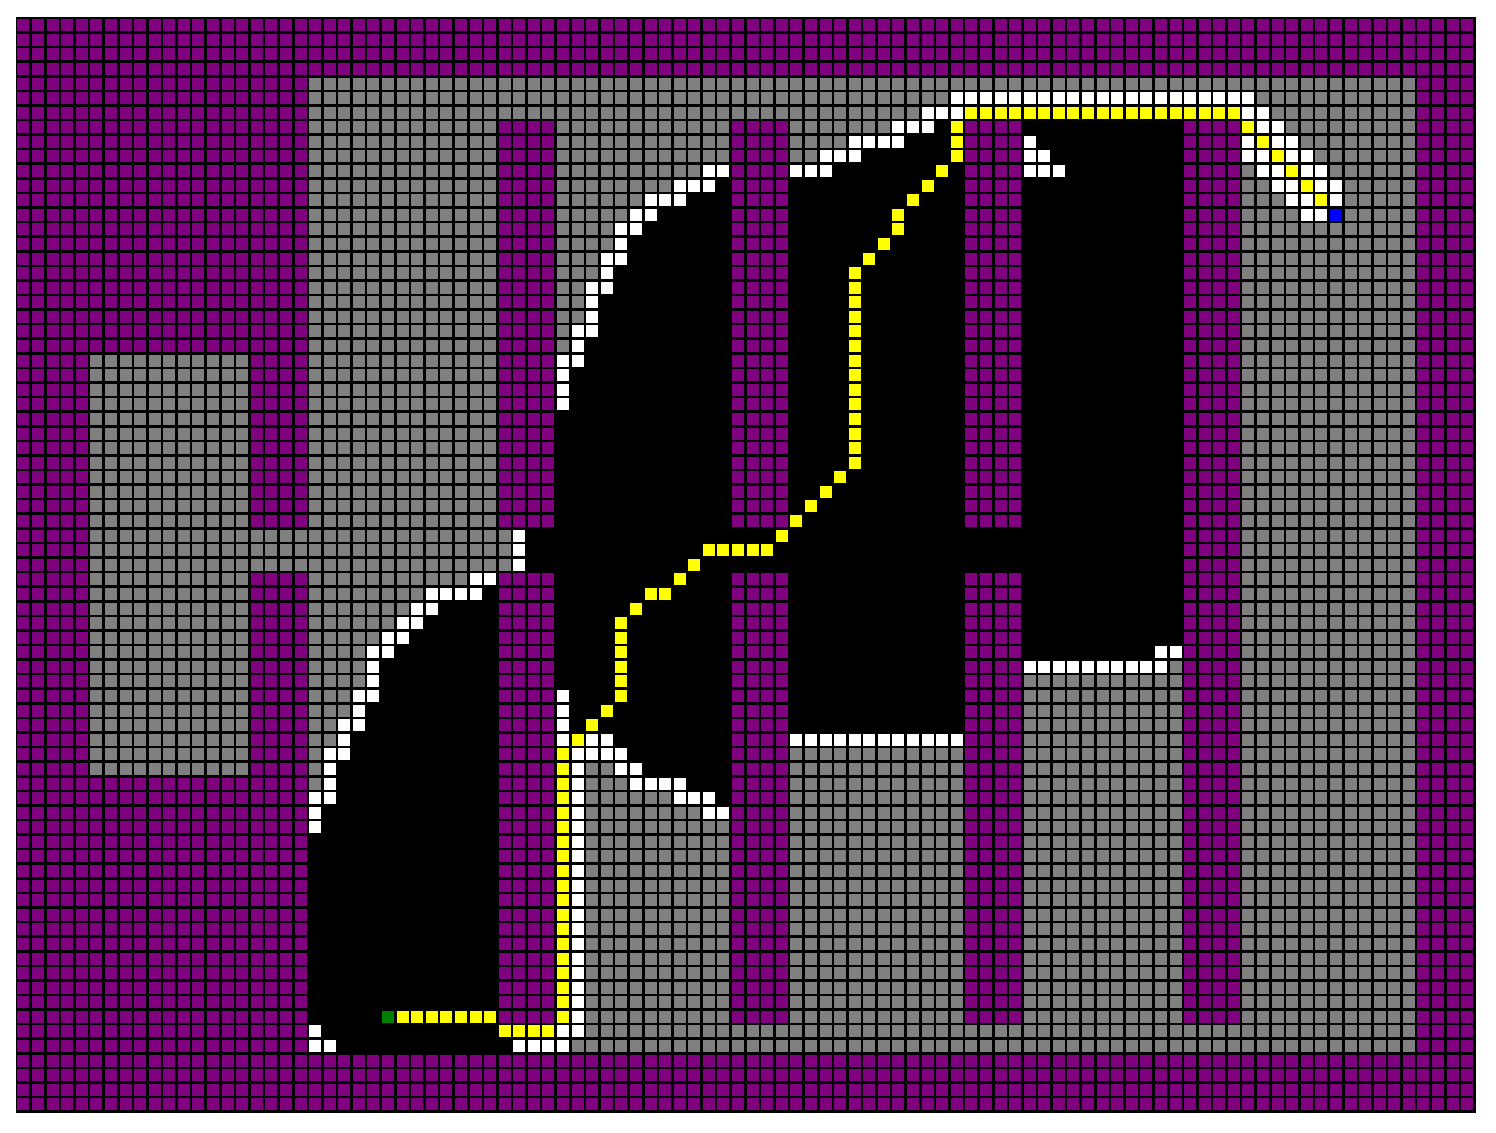
\includegraphics[width=.5\textwidth]{../exports/initial_search_grid_aisleB} 
		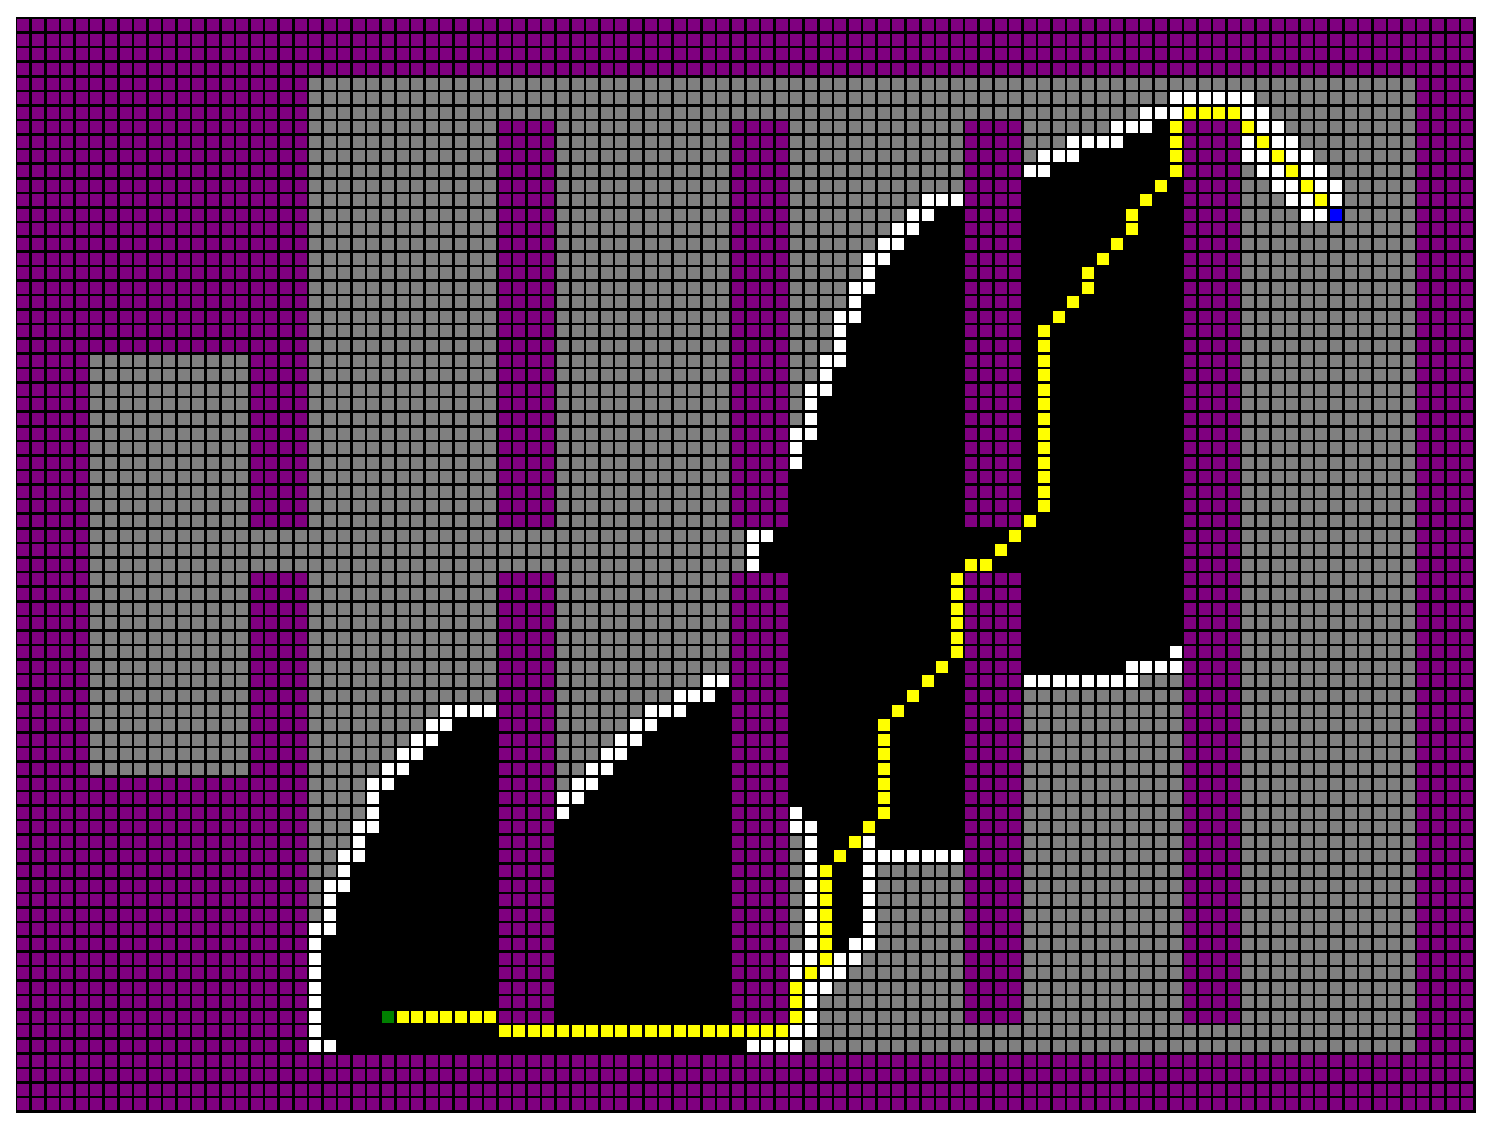
\includegraphics[width=.5\textwidth]{../exports/initial_search_grid_aisleC}
		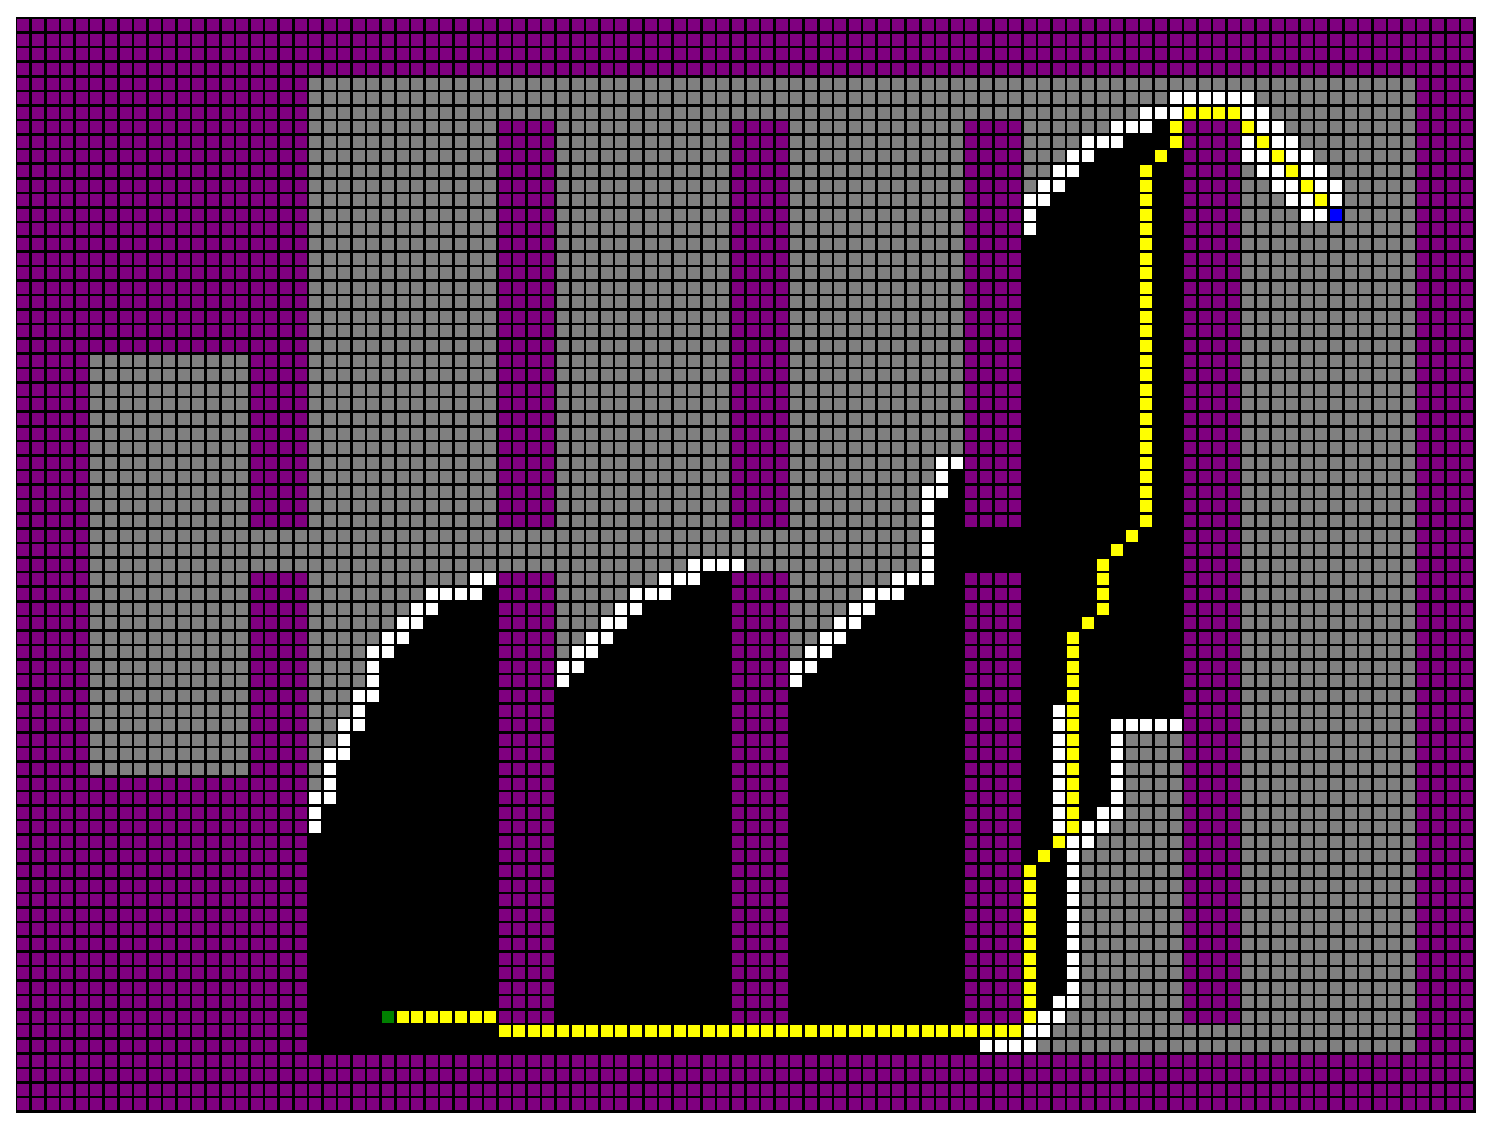
\includegraphics[width=.5\textwidth]{../exports/initial_search_grid_aisleD} 
		\medskip
		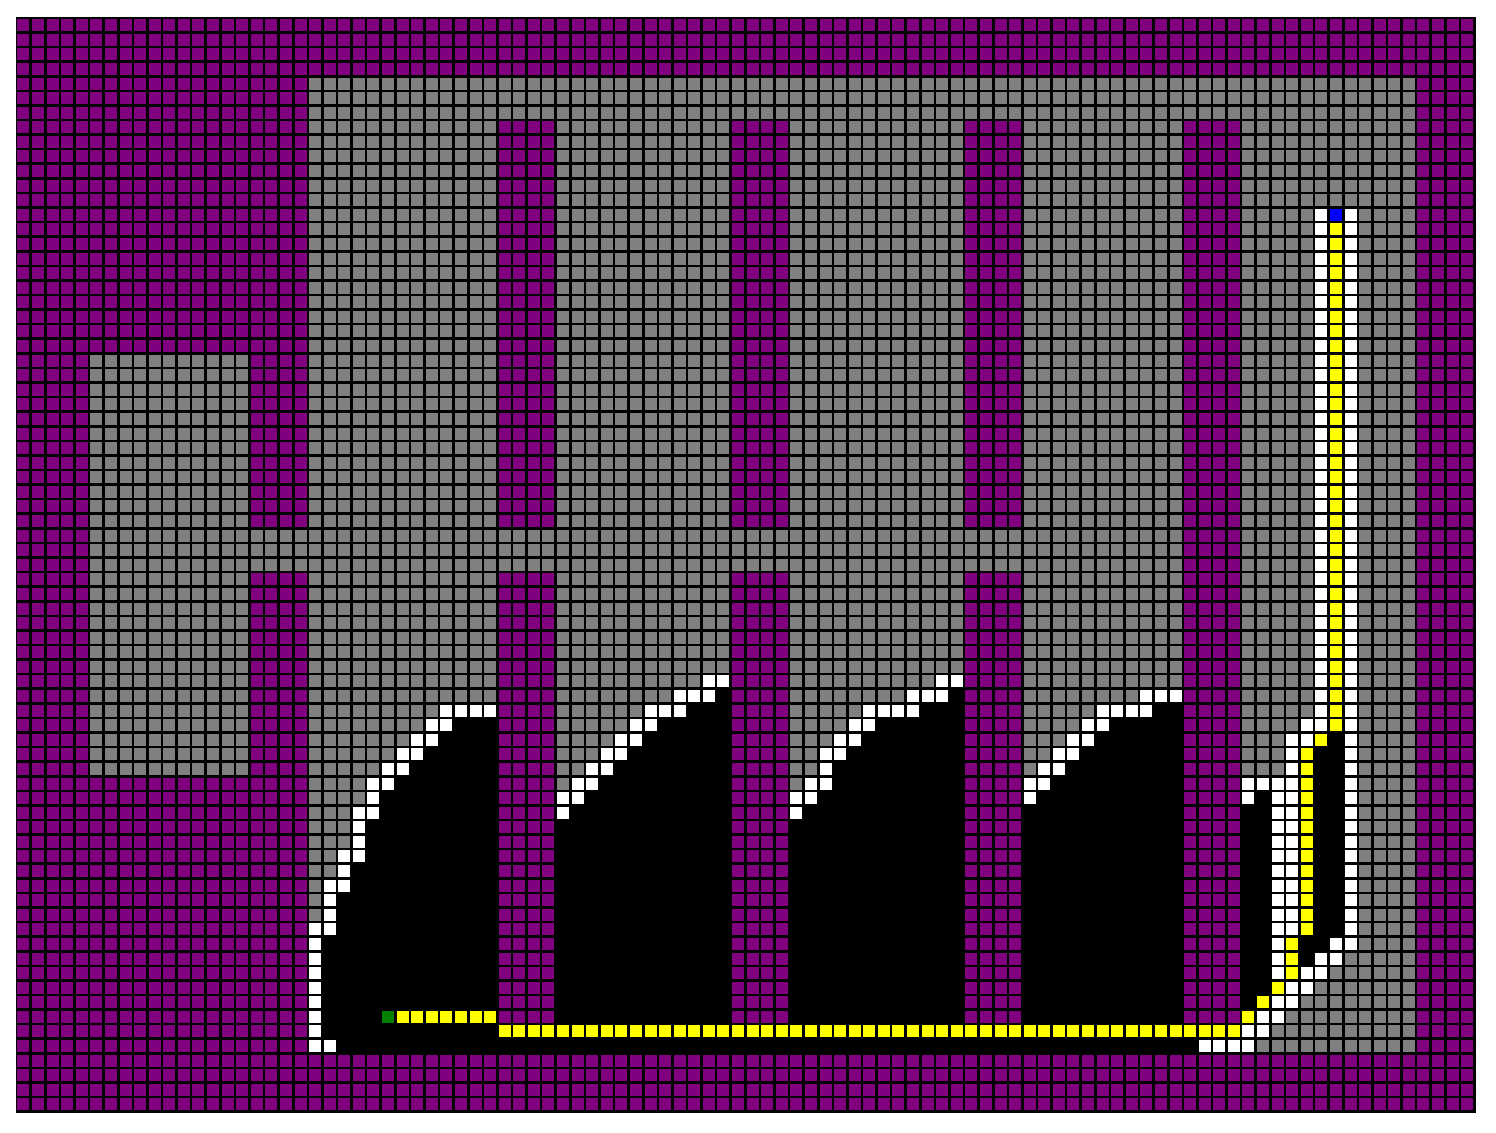
\includegraphics[width=.5\textwidth]{../exports/initial_search_grid_aisleE}
		
		\caption{The demonstration of results of planning via each of the aisles.}
		\label{fig:result-of-plan-via-aisle}
	\end{figure}
	%%%%%%%%%%%%%%%%%%%%%%%%%%%%%%%%%%%%%%
	\newpage
	\bibliographystyle{IEEEtran}
	\bibliography{references}

	%%%%%%%%%%%%%%%%%%%%%%%%%%%%%%%%%%%%%%

	\newpage
	\appendix
	\appendixpage
	\addappheadtotoc
	
\end{document}